\section{Auswertung}
\label{sec:Auswertung}

Die Graphen werden sowohl mit Matplotlib \cite{matplotlib} als auch NumPy \cite{numpy} erstellt. Die Fehlerrechnung wird mithilfe von Uncertainties \cite{uncertainties} durchgeführt.

\subsection{Bestimmung der mittleren Weglänge}

Mit den Werten der Temperaturen $T$ aus Tabelle \ref{tab:w} ergeben sich die mittleren Weglängen $\bar{w}$ nach Formel \eqref{eq:w}. Das Verhältnis $\frac{a}{\bar{w}}$ von $\bar{w}$ zum Abstand $a=\SI{1}{\centi\metre}$ der Kathode zum Gitter ist ebenfalls in der Tabelle eingetragen. Es ist zu erkennen, dass das Verhältnis für $T = \SI{417,15}{\kelvin}$ und für $T = \SI{447,35}{\kelvin}$ dem in der Theorie beschriebenen Wert von $1000-4000$ entspricht, damit die Apparatur für den Franck-Hertz Versuch optimal arbeitet.

\begin{table}
\centering
\caption{Die mittleren Abstände $\bar{w}$ und die Verhältnisse $\frac{a}{\bar{w}}$ für die verschiedenen Temperaturen $T$.}
\label{tab:tabw}
	\sisetup{table-format=1.2}
	\begin{tabular}{S[table-format=3.2]cc}
		\toprule
		{$T/\si{\kelvin}$} & {$\bar{w}/\si{\metre}$} & {$\frac{a}{\bar{w}}$} \\
		\midrule
		 296,65 & 6,14$\cdot10^{-3}$ & 1,63$\cdot10^{0}$ \\
		 417,15 & 7,60$\cdot10^{-6}$ & 1,32$\cdot10^{3}$ \\
		 447,35 & 2,50$\cdot10^{-6}$ & 4,01$\cdot10^{3}$ \\
		 381,15 & 3,60$\cdot10^{-5}$ & 2,77$\cdot10^{2}$ \\
		\bottomrule
	\end{tabular}

\label{tab:w}
\end{table}

\subsection{Bestimmung der Umrechnungsfaktoren}

Für die X-Achse der Graphen aus den Abbildungen \ref{fig:a1} bis \ref{fig:c} werden die Umrechnungsfaktoren bestimmt.
Mit den Werten aus Tabelle \ref{tab:Abstände} und der Formel für den Mittelwert
\[
\mu_d = \frac{1}{N}\sum_i d_i
\]
und der Standardabweichung
\[
\sigma_d = \sqrt{\frac{1}{N^2-N}\sum_i \left(d_i-\mu_d\right)^2}
\]
ergeben sich die mittleren Abstände $\bar{d}$ pro Volt zu:
\begin{align*}
\bar{d}_.{a1} &= \SI{24.8(4)}{\milli\metre\per\volt}\text{,}\\
\bar{d}_.{a2} &= \SI{25.1(4)}{\milli\metre\per\volt}\text{,}\\
\bar{d}_.{b}  &= \SI{4.6(2)}{\milli\metre\per\volt}\text{,}\\
\bar{d}_.{c}  &= \SI{7.7(2)}{\milli\metre\per\volt}\text{.}
\end{align*}
Daraus folgen die Umrechnungsfaktoren $f=\frac{1}{\bar{d}}$ zu:
\begin{align}
f_.{a1} &= \SI{40.3(6)e-3}{\volt\per\milli\per\metre}\text{,}\label{eq:fa1}\\
f_.{a2} &= \SI{39.8(6)e-3}{\volt\per\milli\per\metre}\text{,}\label{eq:fa2}\\
f_.{b}  &= \SI{217(9)e-3}{\volt\per\milli\per\metre}\text{,}\label{eq:fb}\\
f_.{c}  &= \SI{130(3)e-3}{\volt\per\milli\per\metre}\text{.}\label{eq:fc}
\end{align}
Der Fehler $\sigma_{f}$ zu $f$ berechnet sich dabei mit der Gaußschen Fehlerfortpflanzung nach:
\[
\sigma_{f} = \sqrt{\left(\frac{1}{d^2}\right)^2\sigma_d^2} = \frac{1}{d^2}\sigma_d
\]
Dabei ist $\sigma_d$ der Fehler von $d$.

\begin{table}
\centering
\caption{Die Abstände $d$ pro Volt der X-Achse der Graphen aus den Abbildungen \ref{fig:a1}, \ref{fig:a2}, \ref{fig:b} und \ref{fig:c}. Dabei gehört $d_.{a1}$ zu Abbildung \ref{fig:a1}, $d_.{a2}$ zu Abbildung \ref{fig:a2}, $d_.{b}$ zu Abbildung \ref{fig:b} und $d_.{c}$ zu Abbildung \ref{fig:c}.}
\label{tab:tabAbstaende}
	\sisetup{table-format=1.2}
	\begin{tabular}{S[table-format=2.0]S[table-format=2.0]S[table-format=1.1]S[table-format=1.1]}
		\toprule
		{$d_\text{a1}/(\si{\milli\metre\per\volt})$} & {$d_\text{a2}/(\si{\milli\metre\per\volt})$} & {$d_\text{b}/(\si{\milli\metre\per\volt})$} & {$d_\text{c}/(\si{\milli\metre\per\volt})$} \\
		\midrule
		24 & 25 & 4.8 & 8.6 \\
		25 & 24 & 3.6 & 8.0 \\
		23 & 26 & 4.4 & 7.0 \\
		26 & 24 & 4.8 & 7.0 \\
		24 & 23 & 5.6 & 7.0 \\
		23 & 26 & 4.6 & 8.0 \\
		25 & 25 & 4.6 & 8.2 \\
		26 & 26 & 3.6 & 7.8 \\
		26 & 26 & 5.6 & 7.8 \\
		26 & 26 & 4.8 & 7.4 \\
		 {-}  &  {-}  & 4.4 &  {-}  \\
		\bottomrule
	\end{tabular}

\label{tab:Abstände}
\end{table}

\subsection{Bestimmung der Energieverteilung der Elektronen}

In den Abbildungen \ref{fig:a1} und \ref{fig:a2} ist die Integrale Energieverteilung der Elektronen bei $T = \SI{296,65}{\kelvin}$ und $T = \SI{417,15}{\kelvin}$ bei einer konstanten Beschleunigungsspannung von $U_.B = \SI{11}{\volt}$ aufgezeichnet.
In den Abbildungen \ref{fig:1} und \ref{fig:2} sind mit den Werten aus Tabelle \ref{tab:Energieverteilung} die zugehörigen nicht normierten Energieverteilungen angedeutet. Die Spannungen $U_.{A1}$ und $U_.{A2}$ berechnen sich dabei mit den Umrechnungsfaktoren $f_.{a1}$ \eqref{eq:fa1} und $f_.{a2}$ \eqref{eq:fa2}. Der Fehler der Umrechnungsfaktoren wird hierbei vernachlässigt.\\  
Mithilfe des Peaks aus Abbildung \ref{fig:1} bei $U_.P = \SI{8,9(1)}{\volt}$ lässt sich das Kontaktpotential $K_.A$ bestimmen zu:
\[
K_.A = U_.B-U_.P = \SI{2,1(1)}{\volt}\text{.}
\]
Der Fehler $\sigma_{U_.P}$ von $U_.P$ und damit auch von $K_.A$ bestimmt sich nach der Gaußschen Fehlerfortpflanzung nach:
\[
\sigma_{U_.P} = \sqrt{a_.P^2\sigma_{f_.{a1}}^2} = a_.P\sigma_{f_.{a1}}\text{.}
\]
Dabei ist $\sigma_{f_.{a1}}$ der Fehler von $f_.{a1}$ und $a_.P = \SI{221}{\milli\metre}$ der von der Skala abgelesene Abstand.        

\begin{figure}
\centering
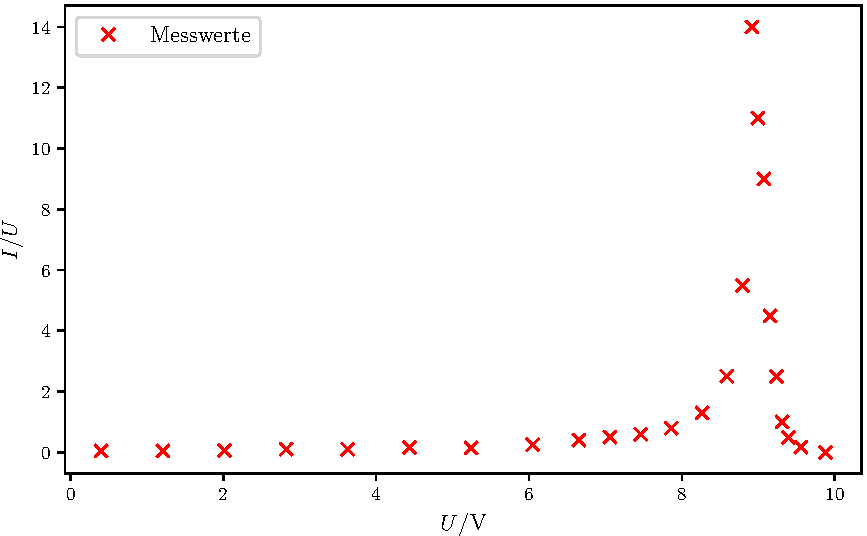
\includegraphics[width=\linewidth-70pt,height=\textheight-70pt,keepaspectratio]{content/images/fig1.pdf}
\caption{Die nicht normierte Energieverteilung der Elektronen bei einer Temperatur von $T=\SI{296,65}{\kelvin}$ und einer Beschleunigungsspannung von $U_.B=\SI{11}{\volt}$.}
\label{fig:1}
\end{figure}

\begin{figure}
\centering
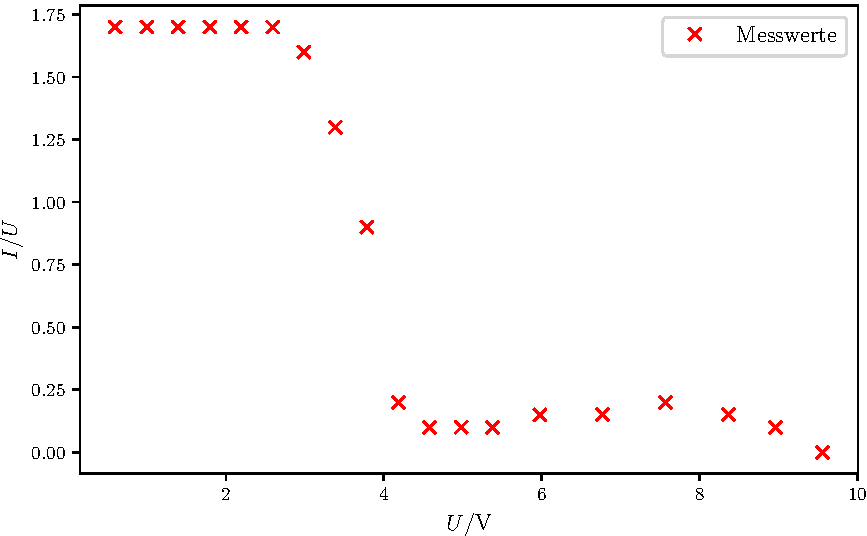
\includegraphics[width=\linewidth-70pt,height=\textheight-70pt,keepaspectratio]{content/images/fig2.pdf}
\caption{Die nicht normierte Energieverteilung der Elektronen bei einer Temperatur von $T=\SI{417,15}{\kelvin}$ und einer Beschleunigungsspannung von $U_.B=\SI{11}{\volt}$.}
\label{fig:2}
\end{figure}

\begin{figure}
\centering
\includegraphics[width=\linewidth-70pt,height=\textheight-70pt,keepaspectratio]{content/images/figure_a1.jpg}
\caption{Die integrale Energieverteilung der Elektronen bei einer Temperatur von $T=\SI{296,65}{\kelvin}$ und einer Beschleunigungsspannung von $U_.B=\SI{11}{\volt}$.}
\label{fig:a1}
\end{figure}

\begin{figure}
\centering
\includegraphics[width=\linewidth-70pt,height=\textheight-70pt,keepaspectratio]{content/images/figure_a2.jpg}
\caption{Die integrale Energieverteilung der Elektronen bei einer Temperatur von $T=\SI{417,15}{\kelvin}$ und einer Beschleunigungsspannung von $U_.B=\SI{11}{\volt}$.}
\label{fig:a2}
\end{figure}

\begin{table}
\centering
\caption{Die Steigung $I_1/U_.{A1}$ zu $U_.{A1}$ abgelesen aus Abbildung \ref{fig:a1} und die Steigung $I_2/U_.{A2}$ zu $U_.{A2}$ abgelesen aus Abbildung \ref{fig:a2}.}
\label{tab:tabEnergieverteilung}
	\sisetup{table-format=1.2}
	\begin{tabular}{S[table-format=1.2]S[table-format=2.2]S[table-format=1.2]S[table-format=1.2]}
		\toprule
		{$U_.{A1}/\si{\volt}$} & {$I_1/U_.{A1}$} & {$U_.{A2}/\si{\volt}$} & {$I_2/U_.{A2}$} \\
		\midrule
		0.40 & 0.05 & 0.60 & 1.70 \\
		1.21 & 0.05 & 1.00 & 1.70 \\
		2.02 & 0.05 & 1.39 & 1.70 \\
		2.82 & 0.10 & 1.79 & 1.70 \\
		3.63 & 0.10 & 2.19 & 1.70 \\
		4.44 & 0.15 & 2.59 & 1.70 \\
		5.24 & 0.15 & 2.99 & 1.60 \\
		6.05 & 0.25 & 3.39 & 1.30 \\
		6.65 & 0.40 & 3.78 & 0.90 \\
		7.06 & 0.50 & 4.18 & 0.20 \\
		7.46 & 0.60 & 4.58 & 0.10 \\
		7.86 & 0.80 & 4.98 & 0.10 \\
		8.27 & 1.30 & 5.38 & 0.10 \\
		8.59 & 2.50 & 5.98 & 0.15 \\
		8.79 & 5.50 & 6.77 & 0.15 \\
		8.91 & 14.00 & 7.57 & 0.20 \\
		8.99 & 11.00 & 8.37 & 0.15 \\
		9.07 & 9.00 & 8.96 & 0.10 \\
		9.15 & 4.50 & 9.56 & 0.00 \\
		9.23 & 2.50 &  {-}  &  {-}  \\
		9.31 & 1.00 &  {-}  &  {-}  \\
		9.40 & 0.50 &  {-}  &  {-}  \\
		9.56 & 0.17 &  {-}  &  {-}  \\
		9.88 & 0.00 &  {-}  &  {-}  \\
		\bottomrule
	\end{tabular}

\label{tab:Energieverteilung}
\end{table}

\subsection{Bestimmung der ersten Anregungsenergie von Quecksilber}

Mithilfe der Werte aus Tabelle \ref{tab:FranckHertz} wird eine lineare Ausgleichsrechnung der Form \newline $U = \alpha n+\beta$ durchgeführt:
\begin{align*}
\alpha = \SI{4,92(2)}{\volt}\text{,}\\
\beta = \SI{0.12(1)}{\volt}\text{.}
\end{align*}
Es ergibt sich eine Anregungsenergie $E_1 = .e\alpha$ von:
\[
E_1 = \SI{4,92(2)}{\electronvolt}\text{.}
\]
Dabei ist $e$ \cite{nistgov} die Elementarladung. Für die Wellenlänge $\lambda$ folgt:
\[
\lambda = \frac{hc}{E_1} = \SI{252(1)}{\nano\metre}\text{.}
\]
Der Fehler $\sigma_\lambda$ von $\lambda$ berechnet sich dabei nach der Gaußschen Fehlerfortpflanzung zu:
\[
\sigma_\lambda = \sqrt{\left(\frac{hc}{E_1^2}\right)^2\sigma_{E_1}^2} = \frac{hc}{E_1^2}\sigma_{E_1} \text{.}
\]
Dabei ist $\sigma_{E_1}$ der Fehler von $E_1$.
Der Energieverlust der Elektronen bei dem zentralen elastischen Stoß muss nicht berücksichtigt werden, da diese die Peaks in Abbildung \ref{fig:b} zwar verwaschen, die Abstände zwischen ihnen jedoch nicht beeinflussen. Zur Berechnung der Spannungen in Tabelle \ref{tab:FranckHertz} wird der Umrechnungsfaktor $f_.b$ \eqref{eq:fb} genutzt, wobei der Fehler vernachlässigt wird. 

\begin{figure}
\centering
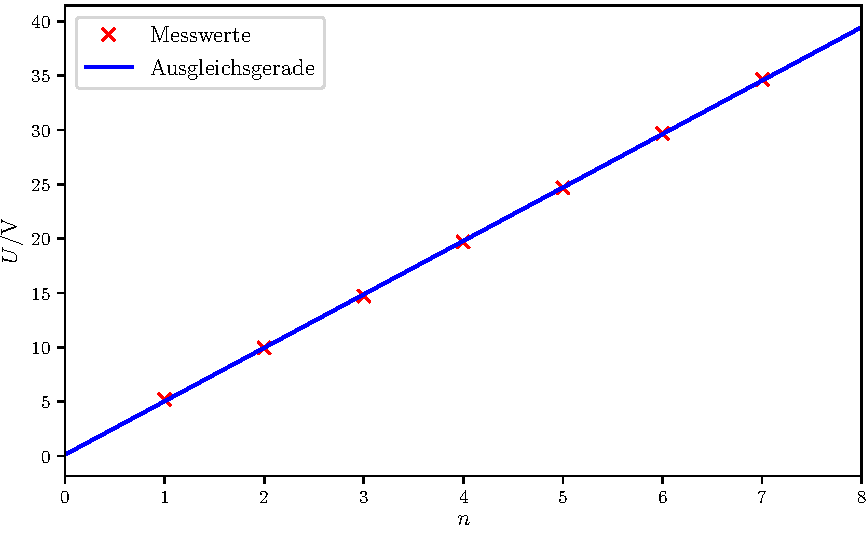
\includegraphics[width=\linewidth-70pt,height=\textheight-70pt,keepaspectratio]{content/images/fig3.pdf}
\caption{Der Wert der Beschleunigungsspannung $U_.B$ des $n$-ten Peaks aufgetragen gegen $n$ bei einer Temperatur von $T=\SI{447,35}{\kelvin}$ und einer Gegenspannung von $U_.A=\SI{1}{\volt}$.}
\label{fig:3}
\end{figure}

\begin{figure}
\centering
\includegraphics[width=\linewidth-70pt,height=\textheight-70pt,keepaspectratio]{content/images/figure_b.jpg}
\caption{Die Franck-Hertz-Kurve bei einer Temperatur von $T=\SI{447,35}{\kelvin}$ und einer Gegenspannung von $U_.A=\SI{1}{\volt}$.}
\label{fig:b}
\end{figure}

\begin{table}
\centering
\caption{Die Werte der Spannung $U_.B$ des $n$-ten Peaks abgelesen aus Abbildung \ref{fig:b}.}
\label{tab:tabFranckHertz}
	\sisetup{table-format=1.2}
	\begin{tabular}{S[table-format=1.0]S[table-format=2.2]}
		\toprule
		{$n$} & {$U_.{B}/\si{\volt}$} \\
		\midrule
		1 & 5.20 \\
		2 & 9.96 \\
		3 & 14.72 \\
		4 & 19.70 \\
		5 & 24.69 \\
		6 & 29.67 \\
		7 & 34.65 \\
		\bottomrule
	\end{tabular}

\label{tab:FranckHertz}
\end{table}

\subsection{Bestimmung der Ionisierungsenergie von Quecksilber}

Zur Bestimmung der Ionisierungsenergie wird der Schnittpunkt der Asymptote an den Graphen in Abbildung \ref{fig:c} betrachtet.
Es ergibt sich mit $a_.{S1} = \SI{136}{\milli\metre}$ ein Schnittpunkt von:
\[
U_.{S1} = a_.{S1}f_.c = \SI{17.7(4)}{\volt}\text{.}
\]
Unter großzügiger Auslegung der Asymptote ergibt sich mit $a_.{S2} = \SI{115}{\milli\metre}$:
\[
U_.{S2} = a_.{S2}f_.c = \SI{15.0(3)}{\volt}\text{.}
\]
Dabei werden die Spannungen mit dem Umrechnungsfaktor $f_.c$ \eqref{eq:fc} aus den abgelesenen Abständen $a_.S$ berechnet. Der Fehler $\sigma_{U_.S}$ zu $U_.S$ folgt nach der Gaußschen Fehlerfortpflanzung:
\[
\sigma_{U_.S} = \sqrt{a_.S^2\sigma_{f_.{c}}^2} = a_.S\sigma_{f_.{c}}\text{.}
\]
Dabei ist $\sigma_{f_.{c}}$ der Fehler von $f_.{c}$.
Somit folgt für die Ionisierungsenergie $E_.{Io} = e(U_.S-K_.A)$:
\begin{align*}
E_.{Io1} = \SI{15.6(4)}{\electronvolt}\text{,}\\
E_.{Io2} = \SI{12.9(4)}{\electronvolt}\text{.}
\end{align*}

\begin{figure}
\centering
\includegraphics[width=\linewidth-70pt,height=\textheight-70pt,keepaspectratio]{content/images/figure_c.jpg}
\caption{Der gemessene Ionenstrom in Abhängigkeit von der Beschleunigungsspannung bei einer Temperatur von $T=\SI{381,15}{\kelvin}$ und einer Gegenspannung von $U_.A=\SI{30}{\volt}$.}
\label{fig:c}
\end{figure}